%\RequirePackage{currfile}
\documentclass[12pt]{beamer}
\usepackage[utf8]{inputenc}
\usepackage[spanish]{babel}
\usepackage{standalone}
\usepackage{color}
\usepackage{siunitx}
\usepackage{hyperref}
\usepackage[outdir=./]{epstopdf}
%\hypersetup{colorlinks,linkcolor=,urlcolor=blue}
%\hypersetup{colorlinks,urlcolor=blue}
\usepackage{xcolor,soul}
\usepackage{etoolbox}
\usepackage{amsmath}
\usepackage{amsthm}
\usepackage{mathtools}
\usepackage{tcolorbox}
\usepackage{physics}
\usepackage{multicol}
\usepackage{bookmark}
\usepackage{longtable}
\usepackage{listings}
\usepackage{cancel}
\usepackage{wrapfig}
\usepackage{empheq}
\usepackage{graphicx}
\usepackage{tikz}
\usepackage{tikz-3dplot}
\usetikzlibrary{calc, patterns, matrix, backgrounds, decorations,shapes, arrows.meta}
\usepackage[autostyle,spanish=mexican]{csquotes}
\usepackage[os=win]{menukeys}
\usepackage{pifont}
\usepackage{pbox}
\usepackage{bm}
\usepackage{caption}
\captionsetup{font=scriptsize,labelfont=scriptsize}
%\usepackage[sfdefault]{roboto}  %% Option 'sfdefault' only if the base font of the document is to be sans serif

%Sección de definición de colores
\definecolor{ao}{rgb}{0.0, 0.5, 0.0}
\definecolor{bisque}{rgb}{1.0, 0.89, 0.77}
\definecolor{amber}{rgb}{1.0, 0.75, 0.0}
\definecolor{armygreen}{rgb}{0.29, 0.33, 0.13}
\definecolor{alizarin}{rgb}{0.82, 0.1, 0.26}
\definecolor{cadetblue}{rgb}{0.37, 0.62, 0.63}
\definecolor{deepblue}{rgb}{0,0,0.5}
\definecolor{brown}{rgb}{0.59, 0.29, 0.0}
\definecolor{OliveGreen}{rgb}{0,0.25,0}
\definecolor{mycolor}{rgb}{0.122, 0.435, 0.698}

\newcommand*{\boxcolor}{orange}
\makeatletter
\newcommand{\boxedcolor}[1]{\textcolor{\boxcolor}{%
\tikz[baseline={([yshift=-1ex]current bounding box.center)}] \node [rectangle, minimum width=1ex, thick, rounded corners,draw] {\normalcolor\m@th$\displaystyle#1$};}}
 \makeatother

 \newcommand*\widefbox[1]{\fbox{\hspace{2em}#1\hspace{2em}}}

\newtcbox{\mybox}{on line,
  colframe=mycolor,colback=mycolor!10!white,
  boxrule=0.5pt,arc=4pt,boxsep=0pt,left=6pt,right=6pt,top=6pt,bottom=6pt}

\usefonttheme[onlymath]{serif}
%Sección de definición de nuevos comandos

\newcommand*{\TitleParbox}[1]{\parbox[c]{1.75cm}{\raggedright #1}}%
\newcommand{\python}{\texttt{python}}
\newcommand{\textoazul}[1]{\textcolor{blue}{#1}}
\newcommand{\azulfuerte}[1]{\textcolor{blue}{\textbf{#1}}}
\newcommand{\funcionazul}[1]{\textcolor{blue}{\textbf{\texttt{#1}}}}
\newcommand{\ptilde}[1]{\ensuremath{{#1}^{\prime}}}
\newcommand{\stilde}[1]{\ensuremath{{#1}^{\prime \prime}}}
\newcommand{\ttilde}[1]{\ensuremath{{#1}^{\prime \prime \prime}}}
\newcommand{\ntilde}[2]{\ensuremath{{#1}^{(#2)}}}
\renewcommand{\arraystretch}{1.5}

\newcounter{saveenumi}
\newcommand{\seti}{\setcounter{saveenumi}{\value{enumi}}}
\newcommand{\conti}{\setcounter{enumi}{\value{saveenumi}}}
\renewcommand{\rmdefault}{cmr}% cmr = Computer Modern Roman

\linespread{1.5}

\usefonttheme{professionalfonts}
%\usefonttheme{serif}
\DeclareGraphicsExtensions{.pdf,.png,.jpg}

%Sección para el tema de beamer, con el theme, usercolortheme y sección de footers
\mode<presentation>
{
  \usetheme{Montpellier}
  
  %\useoutertheme{infolines}
  \useoutertheme{default}
  \usecolortheme{default}
  \setbeamercovered{invisible}
  % or whatever (possibly just delete it)
  \setbeamertemplate{section in toc}[sections numbered]
  \setbeamertemplate{subsection in toc}[subsections numbered]
  \setbeamertemplate{subsection in toc}{\leavevmode\leftskip=3.2em\rlap{\hskip-2em\inserttocsectionnumber.\inserttocsubsectionnumber}\inserttocsubsection\par}
  \setbeamercolor{section in toc}{fg=blue}
  \setbeamercolor{subsection in toc}{fg=blue}
  \setbeamercolor{frametitle}{fg=blue}
  \setbeamertemplate{caption}[numbered]

  \setbeamertemplate{footline}
  \beamertemplatenavigationsymbolsempty
  \setbeamertemplate{headline}{}
}

\makeatletter
\setbeamercolor{section in foot}{bg=gray!30, fg=black!90!orange}
\setbeamercolor{subsection in foot}{bg=blue!30!yellow, fg=red}
\setbeamertemplate{footline}
{
  \leavevmode%
  \hbox{%
  \begin{beamercolorbox}[wd=.333333\paperwidth,ht=2.25ex,dp=1ex,center]{section in foot}%
    \usebeamerfont{section in foot} \insertsection
  \end{beamercolorbox}}%
  \begin{beamercolorbox}[wd=.333333\paperwidth,ht=2.25ex,dp=1ex,center]{subsection in foot}%
    \usebeamerfont{subsection in foot}  \insertsubsection
  \end{beamercolorbox}%
  \begin{beamercolorbox}[wd=.333333\paperwidth,ht=2.25ex,dp=1ex,right]{date in head/foot}%
    \usebeamerfont{date in head/foot} \insertshortdate{} \hspace*{2em}
    \insertdate{\today} \hspace{0.3cm} \insertframenumber{} / \inserttotalframenumber \hspace*{2ex} 
  \end{beamercolorbox}}%
  \vskip0pt%
\makeatother  

\makeatletter
\patchcmd{\beamer@sectionintoc}
  {\vfill}
  {\vskip\itemsep}
  {}
  {}
\makeatother


\title{\large{Minimizando el error de interpolación}}
\subtitle{Polinomios de Chebychev}
\author{M. en C. Gustavo Contreras Mayén}
\date{}
\institute{Facultad de Ciencias - UNAM}
\titlegraphic{
\includegraphics[width=1.75cm]{../Imagenes/escudo-facultad-ciencias}\hspace*{4.75cm}~%
   
\includegraphics[width=1.75cm]{../Imagenes/escudo-unam}
}
\setbeamertemplate{navigation symbols}{}
\begin{document}
\maketitle
\fontsize{14}{14}\selectfont
\spanishdecimal{.}
\section*{Contenido}
\frame[allowframebreaks]{\tableofcontents[currentsection, hideallsubsections]}
\section{Las raíces de Chebychev}
\frame{\tableofcontents[currentsection, hideothersubsections]}
\subsection{Interpretación geométrica}
\begin{frame}
\frametitle{Raíces del polinomio Chebychev}
Una interpretación geométrica de las raíces de Chebychev es aquella según la cual estos se colocan en un segmento de longitud igual al diámetro de un círculo, cuya circunferencia repartimos en $n$ partes iguales.
\end{frame}
\begin{frame}
\frametitle{Raíces del polinomio Chebychev}
Proyectando a lo largo del dicho segmento el punto medio de cada partición de la semicirconferencia obtenemos puntos que coinciden con las raíces del polinomio de Chebychev.
\begin{figure}
    \centering
    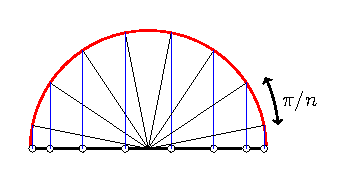
\includegraphics[scale=1]{Imagenes/Nodos_Chebychev_01.eps}
\end{figure}
\end{frame}
\begin{frame}
\frametitle{Minimizando el efecto Runge}
La razón por la cual la aproximación de una función $f(x)$ por un polinomio que interpole puntos escogidos de esta forma minimiza el efecto Runge es que la densidad de puntos resulta creciente desde el centro hasta los extremos.
\end{frame}
\begin{frame}
\frametitle{Minimizando el efecto Runge}
Para calcular dichas raices utiliza la identidad trigonométrica del polinomio de Chebychev:
\begin{align*}
T_{n}(x) = \cos (n \, \arccos x) = \cosh (n \, \mbox{arccosh} \, x)
\end{align*}
\pause
Este coseno se anula cuando la expresión al interior es un múltiplo de $2 \, \pi$.
\end{frame}
\begin{frame}
\frametitle{Raíces polinomio Chebychev}
Por lo tanto las raíces del polinomio de Chebychev en $[-1,1]$ son:
\begin{align*}
x_{i} = \cos \left( \dfrac{2 \, i - 1}{2 \, n} \, \pi \right) \hspace{1cm} i = 1, 2, \ldots, n
\end{align*}
\end{frame}
\begin{frame}
\frametitle{Raíces polinomio Chebychev}
En el caso de que se quisiera definir el polinomio de Chebychev en un intervalo cualquiera $[a, b]$, las raíces se trasforman como:
\begin{align*}
x_{i} = \dfrac{a + b}{2} &+ \dfrac{b - a}{2} \, \cos \left( \dfrac{2 \, i - 1}{2 \, n} \, \pi \right) \\[0.5em] 
i =& 0, 1, \ldots, n
\end{align*}
\end{frame}
\begin{frame}
\frametitle{Obteniendo coeficientes}
La utilización de los nodos de Chebychev nos permite también utilizar un método recursivo para la obtención de los coeficientes:
\begin{align*}
f(x) \simeq \sum_{j=0}^{n} c_{j} \, T_{j}(x)
\end{align*}
donde los coeficientes $c_{j}$ son:
\end{frame}
\begin{frame}
\frametitle{Obteniendo coeficientes}
Los coeficientes $c_{j}$ son:
\begin{align*}
c_{0} &= \dfrac{1}{n + 1} \, \sum_{j=0}^{n} f(x_{k}) \, T_{0}(x_{k}) = \dfrac{1}{n + 1} \, \sum_{j=0}^{n} f(x_{k}) \\[0.5em]
c_{j} &= \dfrac{1}{n + 1} \, \sum_{j=0}^{n} f(x_{k}) \, T_{j}(x_{k})
\end{align*}
\end{frame}
\begin{frame}
\frametitle{Usando los coeficientes}
Esta fórmula permita calcular los coeficientes del polinomio de interpolación con un costo computacional del orden de $\order{n^{2}}$ operaciones.
\end{frame}
\section{Ejercicio}
\frame{\tableofcontents[currentsection, hideothersubsections]}
\subsection{Ajuste polinomial}
\begin{frame}
\frametitle{Enunciado}
Consideramos la función:
\begin{align*}
f(x) = \dfrac{800 \, x}{54 \, x^{4} + x^{2} + 3}
\end{align*}
para interpolar dos polinomios de igual grado a los puntos de dicha función, en el intervalo $[-1, 1]$.
\end{frame}
\begin{frame}
\frametitle{Gráfica de la función}
La función a interpolar es la siguiente:
\begin{figure}
    \centering
    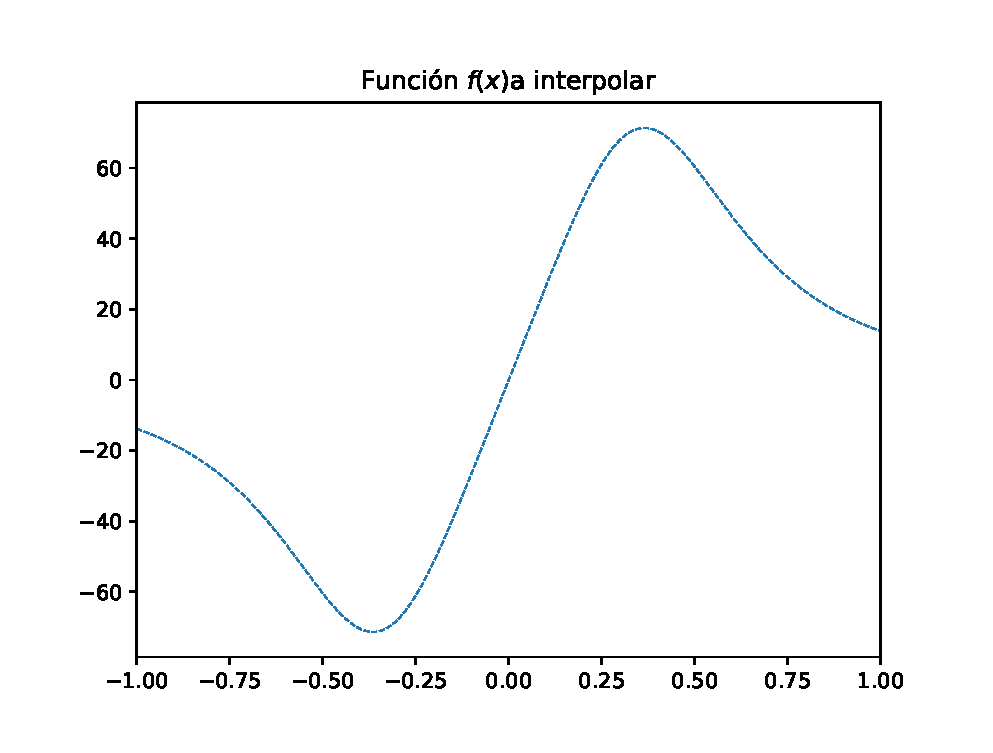
\includegraphics[scale=0.5]{Imagenes/Plot_Ejercicio_Chebychev_01.eps}
\end{figure}
\end{frame}
\begin{frame}
\frametitle{Estrategia}   
El primer polinomio lo interpolamos con puntos equiespaciados y el segundo en las raíces del polinomio de Chebychev.
\\
\bigskip
\pause
Utilizamos dos medidas de distancia para evaluar la bondad de la aproximación:
\end{frame}
\begin{frame}
\frametitle{Evaluando la aproximación}
El error debido a la diferencia del área al cuadrado entre la función y el polinomio de interpolación:
\begin{align*}
d_{1} (f, p) = \int_{a}^{b} \big[ f(x) - p(x) \big]^{2} \dd{x}
\end{align*}
\end{frame}
\begin{frame}
\frametitle{Segundad medida de aproximación}
La segunda medida para medir la bondad de la aproximación es la distancia máxima entre los puntos entre la función y el polinomio de interpolación:
\begin{align*}
d_{2} (f, p) = \max_{x} \abs{f(x) - p(x)}
\end{align*}
\end{frame}
\section{Implementación con python}
\frame{\tableofcontents[currentsection, hideothersubsections]}
\subsection{Usando las librerías de python}
\begin{frame}
\frametitle{Usando python}
Con la finalidad de ocupar un lenguaje más versátil para resolver el ejercicio, usamos python y las librerías con las cuales podremos obtener los valores de $d_{1}$ y $d_{2}$, así como las gráficas de los procesos de aproximación con los puntos equidistantes y con los puntos de las raíces de los polinomios de Chebychev.
\end{frame}
\begin{frame}
\frametitle{Librerías}
Se han ocupado las siguientes librerías:
\setbeamercolor{item projected}{bg=blue!70!black,fg=yellow}
\setbeamertemplate{enumerate items}[circle]
\begin{enumerate}[<+->]
\item \texttt{numpy.polyfit} y \texttt{numpy.poly1d}.
\item \texttt{scipy.integrate.quad}
\item \texttt{scipy.special.roots\_chebyt}
\item \texttt{matplotlib.pyplot}
\end{enumerate}
\end{frame}
\begin{frame}
\frametitle{Comenzando la solución}
Se calculan $d_{1}$, $d_{2}$, así como las gráficas del ajuste polinomial con puntos equidistantes y con las raíces del polinomio de Chebychev para el conjunto de puntos:
\begin{align*}
n = 3, 5, 8, 10, 12, 14, 16
\end{align*}
que se presentan a continuación:
\end{frame}
\begin{frame}
\frametitle{Con $n = 3$}
    \centering
    \includegraphics<1>[scale=0.625]{Imagenes/Interpolacion_Chebychev_03_Polinomio.eps}% 
    \includegraphics<2>[scale=0.625]{Imagenes/Interpolacion_Chebychev_03_Raices.eps}
\end{frame}
\begin{frame}
\frametitle{Con $n = 5$}
    \centering
    \includegraphics<1>[scale=0.625]{Imagenes/Interpolacion_Chebychev_05_Polinomio.eps}% 
    \includegraphics<2>[scale=0.625]{Imagenes/Interpolacion_Chebychev_05_Raices.eps}
\end{frame}
\begin{frame}
\frametitle{Con $n = 8$}
    \centering
    \includegraphics<1>[scale=0.625]{Imagenes/Interpolacion_Chebychev_08_Polinomio.eps}% 
    \includegraphics<2>[scale=0.625]{Imagenes/Interpolacion_Chebychev_08_Raices.eps}
\end{frame}
\begin{frame}
\frametitle{Con $n = 10$}
    \centering
    \includegraphics<1>[scale=0.625]{Imagenes/Interpolacion_Chebychev_10_Polinomio.eps}% 
    \includegraphics<2>[scale=0.625]{Imagenes/Interpolacion_Chebychev_10_Raices.eps}
\end{frame}
\begin{frame}
\frametitle{Con $n = 12$}
    \centering
    \includegraphics<1>[scale=0.625]{Imagenes/Interpolacion_Chebychev_12_Polinomio.eps}% 
    \includegraphics<2>[scale=0.625]{Imagenes/Interpolacion_Chebychev_12_Raices.eps}
\end{frame}
\begin{frame}
\frametitle{Con $n = 14$}
    \centering
    \includegraphics<1>[scale=0.625]{Imagenes/Interpolacion_Chebychev_14_Polinomio.eps}% 
    \includegraphics<2>[scale=0.625]{Imagenes/Interpolacion_Chebychev_14_Raices.eps}
\end{frame}
\begin{frame}
\frametitle{Con $n = 16$}
    \centering
    \includegraphics<1>[scale=0.625]{Imagenes/Interpolacion_Chebychev_16_Polinomio.eps}% 
    \includegraphics<2>[scale=0.625]{Imagenes/Interpolacion_Chebychev_16_Raices.eps}
\end{frame}
\begin{frame}
\frametitle{Resumen}
\begin{table}
    \fontsize{12}{12}\selectfont
\begin{tabular}{| c | c | c |} \hline
puntos & $d_{1}$ & $d_{2}$ \\\hline
\multirow{2}{*}{$3$} & $3281.06$ & $66.33$ \\
 & $2799.63$ & $62.98$ \\ \hline
 \multirow{2}{*}{$5$} & $709.14$ & $28.11$ \\
 & $714.92$ & $34.66$ \\ \hline 
 \multirow{2}{*}{$8$} & $19.85$ & $5.68$ \\
 & $6.82$ & $4.12$ \\ \hline
\end{tabular}
\end{table}
\end{frame}
\begin{frame}
\frametitle{Resumen}
\begin{minipage}[t]{0.4\textwidth}
\begin{table}
\fontsize{12}{12}\selectfont
\begin{tabular}{| c | c | c |} \hline
puntos & $d_{1}$ & $d_{2}$ \\\hline
\multirow{2}{*}{$10$} & $317.75$ & $37.95$ \\
    & $6.99$ & $3.82$ \\ \hline
    \multirow{2}{*}{$12$} & $478.56$ & $52.64$ \\
    & $3.0$ & $2.31$ \\ \hline 
    \multirow{2}{*}{$14$} & $164.88$ & $35.73$ \\
    & $0.6$ & $1.01$ \\ \hline
\end{tabular}
\end{table}
\end{minipage}
\hspace{1.5cm}
\begin{minipage}[t]{0.4\textwidth}
\begin{table}
\fontsize{12}{12}\selectfont
\begin{tabular}{| c | c | c |} \hline
puntos & $d_{1}$ & $d_{2}$ \\\hline
\multirow{2}{*}{$16$} & $44.12$ & $19.73$ \\
    & $0.05$ & $0.32$ \\ \hline
\end{tabular}
\end{table}
\end{minipage}
\end{frame}
\begin{frame}
\frametitle{Conclusión}
Lo que encontramos claramente es que el método con las raíces del polinomio de Chebychev resulta óptimo para la minimización de la mayor distancia existente entre la función que se desea aproximar $f(x)$ y el polinomio que se construye con las raíces de Chebychev.
\\
\bigskip
\pause
Sin embargo, esto no garantiza de ninguna forma la minimización del otras distancias, como se observó en caso de la norma $d_{1}$.
\end{frame}
\begin{frame}
\frametitle{Conclusión}
Un inconveniente considerable de dicho método es que si queremos añadir más puntos, se tendría que estimar de nuevo los coeficientes de los polinomios de Chebychev.
\\
\bigskip
\pause
Con un algoritmo en python, se simplifica esta tarea ya que el cálculo se realiza nuevamente al modificar el número de puntos $n$, las demás tareas ya quedan establecidas en funciones que se mandan llamar.
\end{frame}
\end{document}